%----------------------------------------------------------------------------------------
%	SLIDE 3.
%----------------------------------------------------------------------------------------
\begin{frame}
\frametitle{Threads, Processes, Cores and other creatures}

\only<1,3-> {
\begin{block}{CPU (\q{Central Processing Unit}) and cores}
	\begin{itemize}
		\item \q{The brain of a computer}, it is responsible for
		\begin{itemize}
			\item the calculation of arithmetic operations,
			\item performing logical operations,
			\item operation of the other hardware components.
		\end{itemize}
		\item Nowadays all CPUs are multi-core
		\begin{itemize}
			\item First multi(two)-core model: POWER4 (IBM, 2001)
		\end{itemize}
	\end{itemize}
\end{block}
}

\only<2> {
\begin{figure}
	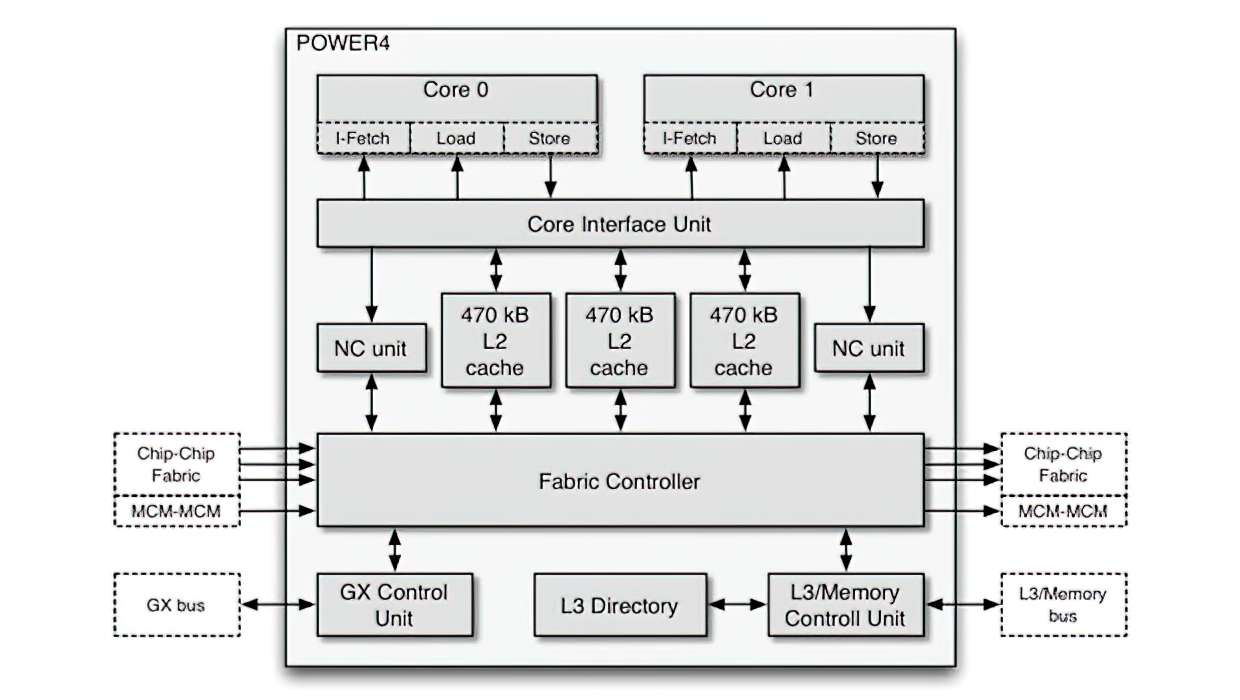
\includegraphics[width=\textwidth]{img/power4-2x.png}
	{\hspace*{\fill}\tiny\textit{Source: ibm.com}}	
\end{figure}
}

\uncover<3-> {
\begin{alertblock}{Processes, Threads}
	\begin{itemize}
		\item Process
		\begin{itemize}
			\item Name for a single, running program
		\end{itemize}
		\item Thread
		\begin{itemize}
			\item A running sequence of operations 
			\item A process can be broken down into several threads
			\item They always run \q{in parallel}
		\end{itemize}
	\end{itemize}
\end{alertblock}
}

\end{frame}